\documentclass[11pt]{article}
\usepackage{amsmath,amssymb,amsthm,amsfonts,hyperref, enumitem, tikz}
\usepackage{algorithm}
\usepackage{algpseudocode}
\usepackage{subfigure}

\title{Puck Predictions: Unraveling the NHL Game Forecasting Riddle}
\author{Jason Vasquez \and Dylan Skinner \and Jeff Hansen \and Benjamin McMullin}

\begin{document}

\maketitle

\begin{abstract}
    The goal of this project is simple: predict the outcomes of NHL games from any given state during the game. To solve this problem we use three primary methods: Bayesian Network to train a DAG, XGBoost on game states, and an MCMC game simulator. We use each of these methods to generate win probabilities for each time step throughout various NHL games, thus emulating a live win probability. Finally, we analyze the accuracy of these three methods and considered ethical implications of our results.
\end{abstract}

\section{Problem Statement and Motivation}
% Your content for this section goes here
In the world of sports analytics, predicting the outcomes of games is a common and challenging problem, with live win predictions adding
an extra layer of complexity. For most sports, there are a plethora of widely accepted—yet hidden—predictive models and methods that are used to
predict games. In addition to this, most sports have easily accessible statistics and graphics that give current win probabilities for any live game.

Hockey, however, is a different story. While there are some methods used to predict the outcome of National Hockey League (NHL) games, these models
typically belong to sport books and their nuances are not publicly disclosed. Additionally, hockey analytics is not as
developed as it is in other sports, such as basketball or baseball. This lack of model transparency and public interest in hockey analytics
makes predicting the outcomes of NHL games a very underdeveloped and challenging problem. Previous attempts and research into predicting NHL games
has relied on methods such as decision trees and artificial neural networks~\cite{pishcedda} (from 2014), naïve bayes and support vector machines~\cite{weissbock2013use} (from 2013),
and Monte Carlo simulations~\cite{Weissbock2014ForecastingSI} (from 2014).

In addition to model research, some research has also gone into developing new features that can be used to better predict the game outcomes. 
The two biggest engineered classes of features are the Corsi
 and Fenwick\footnote{These metrics were created by sports bloggers Tim Barnes and Mark Fenwick, respectively. 
 We were unable to locate the original blog posts talking about these metrics, but a good article to learn more about the math can be
 found here \url{https://thehockeywriters.com/corsi-fenwick-stats-what-are-they/}.} metrics (both around 2007). 

Our project seeks a similar outcome to the research mentioned above: predict the outcomes of NHL games. Not only this,
but we seek to provide live, acturate win probabilities for any given game state. Despite the simplicity of the problem statement, 
as mentioned, the solution is not so straightforward. The NHL provides fast-paced games with many events
occuring in quick succession. Our goal is to use this abundance of data and new approaches to build upon previous research.

Our motivation for this project exists strictly as fans of the sport and as data scientists. Our model is not intended to be used for gambling or any other
nefarious purposes—any use of this model for such purposes is a misuse of our work.

\section{Data}
% Your content for this section goes here
Our data came from the hockeyR Github repository~\cite{hockeyR-data}. This repository contains an abundance of data about every NHL game
that has occured since the 2010-11 season. This data includes information about the events that transpire in a game (hits, shots, goals, etc.),
which teams are playing, who is on the ice, and the final score of the game. The data is stored in a series of {\tt .csv.gz} files, allowing for
easy access and manipulation.

Each game in a season is given a unique identifier ({\tt game\_id}), which is constant across all events in a game. Every event that occurs in a game
will be stored in the {\tt event\_type} column. There are 17 unique event types, including things such as game start, faceoff, shot, hit, and goal.
Most of these event types are not relevant to our analysis, so we remove them from the dataset. After removing the unnecessary events, we are left with
nine events: blocked shot, faceoff, giveaway, goal, hit, missed shot, penalty, shot, and takeaway. These events are attributed to the
team and player that performs the event. We only take into consideration the team that performs the event and discard the player information.

The data also contains information about when the event occured. This appears in a variaty of formats, but we only
use the {\tt game\_time\_remaining} column. {\tt game\_time\_remaining} starts
at 3600 (60 minutes) and counts down to 0. If the game goes into extra time, i.e., it is tied after 60 minutes, {\tt game\_time\_remaining} will
be a negative value.

We found that our data did not contain any missing values that was not easily explainable. For example, if a game is starting, there will be no
events for penalties, which will result in a {\tt NaN} value in the penalties column. Additionally, any data that was confusing or not easily explainable
(for example the home team having 7 players on the ice and the away team having 5), was manually verified by watching a clip of the game where
the event occured to make sure the event was recorded correctly. We did not find any incorrectly recorded events, so we 
did not remove any strange events from out dataset.

\section{Methods}

\subsection{Bayesian Network}
We first used a Bayesian Network to establish a benchmark for probability using several key features.

Bayesian networks are probabilistic graphical models that represent probabilistic relationships among a set of variables using a directed acyclic graph (DAG). 
In a Bayesian network, nodes represent random variables, and directed edges between nodes represent probabilistic dependencies between the variables. Each node in the graph is associated with a conditional probability distribution that quantifies the probability of that variable given its parent variables in the graph.

For our purposes, we predefined the structure of the network, and used the data to calculate the conditional probabilities for each node. We then used the network to calculate the probability of a team winning given the current state of the game.

The computational complexity of Bayesian Network inference is high, with exact inference being an NP-hard problem~\cite{pmlr-vR0-chickering95a}. 
Using the python package pgmpy, we originally tried to fit a network with all 26 of our features, but our computational resources failed to fit this network.
Then, to get a baseline for our future predictions, we simply fitted the model with the base features of time remaining (tr), home goals (hg), away goals (ag), home shots (hs), away shots (as), home blocked shots (hbs), and away blocked shots (abs) in order to predict wins (w). 
These features were chosen as priors because of our opinion that they are the most important to the game, based upon our knowledge of hockey.


The conditional dependencies of the chosen network are shown in the DAG below:

\begin{center}
    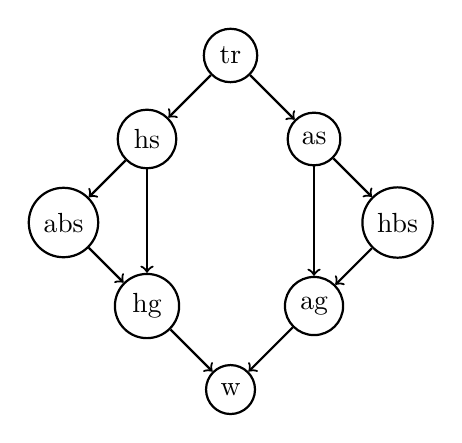
\begin{tikzpicture}[node distance={15mm}, thick, main/.style = {draw, circle}]
        \node[main] (1) {tr}; 
        \node[main] (2) [below left of=1] {hs};
        \node[main] (3) [below right of=1] {as};
        \node[main] (4) [below right of=3] {hbs};
        \node[main] (5) [below left of=2] {abs};
        \node[main] (6) [below right of=5] {hg};
        \node[main] (7) [below left of=4] {ag};
        \node[main] (8) [below left of=7] {w};

        \draw[->] (1) -- (2);
        \draw[->] (1) -- (3);
        \draw[->] (3) -- (4);
        \draw[->] (2) -- (5);
        \draw[->] (5) -- (6);
        \draw[->] (4) -- (7);
        \draw[->] (3) -- (7);
        \draw[->] (2) -- (6); 
        \draw[->] (6) -- (8);
        \draw[->] (7) -- (8);  

    \end{tikzpicture} 
\end{center}

This model was chosen for the task because different stats in hockey are conditionally dependent of each other, so by modeling those conditional
dependencies and feeding them into the model, we can hopefully acheive a more accurate prediction of the outcome of the game.

\subsection{XGBoost}

In our NHL analysis research, we partitioned the dataset into segments 
corresponding to individual teams' games over multiple seasons. 
This enabled the creation of time series data in the form of a state vector, capturing the 
play-by-play dynamics of each team's matches. We then trained 
separate XGBoost models for each team to learn their unique patterns 
and strategies. We chose to create an XGBoost model for each team
because we felt it would be more accurate than a single model for all teams.
This is because some teams do very well and some teams do very poorly, and
we felt this difference necessitated a model for each team.


\subsection{MCMC Game Simulation}

To simulate hockey games, we created a Markov Chain where the states are a tuple of three consecutive
events that occurred. For example, if the home team won a faceoff, the home team lost the puck, and 
then the away team shot the puck and missed, the markov chain would look like figure~\ref{fig:markov_chain_sample}.

\begin{figure}[H]
    \centering
    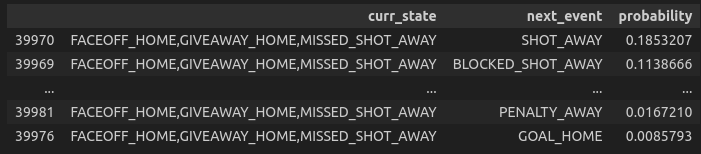
\includegraphics[width=0.8\textwidth]{images/markov_chain_sample.png}
    \caption{Sample Markov Chain for the current state (home team won faceoff, 
    home team lost puck, away team missed shot) with the probabilities of the next event 
    sorted from highest to lowest}
    \label{fig:markov_chain_sample}
\end{figure}

The probabilities of transitioning from one triple-state to another triple-state is calculated by:
\begin{align*}
    P(s_{t+1} = (B,C,D) \;|\; s_t = (A,B,C)) &= P(D \;|\; (A,B,C)) \\
    &= \frac{\{ \text{\# of times (A,B,C,D) happend}\}}{\{ \text{\# of times (A,B,C) happened}\}} \\
\end{align*}
Where $A,B,C,D$ represent events that can occur in a game, and the tuple (A,B,C,D) represents that "A then 
B then C then D" happened right after each other in a game.

To simulate a game, we performed this Monte Carlo algorithm that acted like a random walk through the Markov Chain (Note that the KDE\_times() is a KDE model fit on the amount of seconds that transpired between 
each hockey event for all NHL games over the course of 13 years):
\begin{algorithm}[H]
    \caption{Simulation Algorithm}
    \begin{algorithmic}[1]
        \State $\text{time\_remaining} \gets 3600$
        \Comment{NHL games are 3600 seconds}
        \State $s_0 \gets "\#"$
        \Comment{The "\#" symbol represents the start of a game}
        \State $s_1 \gets "\#"$
        \State $s_2 \gets "\#"$
        \State $\text{event\_counts} \gets \text{dictionary()}$

        \While{$\text{time\_remaining} > 0$}
            \State $\text{next\_state} \gets \text{sample from } \text{MC(curr\_state)}$
            \State $\text{event\_counts}[\text{next\_state}] \mathrel{+}= 1$
            
            \State $s_0 \gets s_1$
            \State $s_1 \gets s_2$
            \State $s_2 \gets \text{next\_state}$

            \State $\text{event\_time} \gets \text{sample from } \text{KDE\_times()}$
            \State $\text{time\_remaining} \gets (\text{time\_remaining} - \text{event\_time})$
        \EndWhile
    \end{algorithmic}
    \label{alg:monte_carlo_algorithm}
\end{algorithm}

To predict a team's winning probability, we would simulate 50 hockey games with the initial starting states $(s_0, s_1, s_2)$ set to the most current events in the hockey game. By looking at each games
final event counts, we could compute each game's winner. Then we computed the 
probability as $P(\text{home winning}) = \{\text{\# home simulation wins}\}/50$ and 
$P(\text{away winning}) = 1-P(\text{home winning})$.

\section{Results and Analysis}
% Your content for this section goes here

\subsection{Bayesian Network}

Overall, the Bayesian Network performed well, and was able to produce realistic win probabilities. Because it defined a joint distribution using a DAG and
then used that distribution to fit the data, it was able to correctly predict accuracies using the few features provided. However, the Bayesian Network struggled to capture the intricate dependencies
of factors other than goals that could affect the win probabilities, so the predicted probabilities are little more than an over probability calculation of goals and time reamining given historical data.
We see this in the probability graph below, where the changes in probability correspond to the goals scored in the game. A sample win probability graph is seen below in ~\ref{fig:bayesian_graph}

\begin{figure}[H]
    \centering
    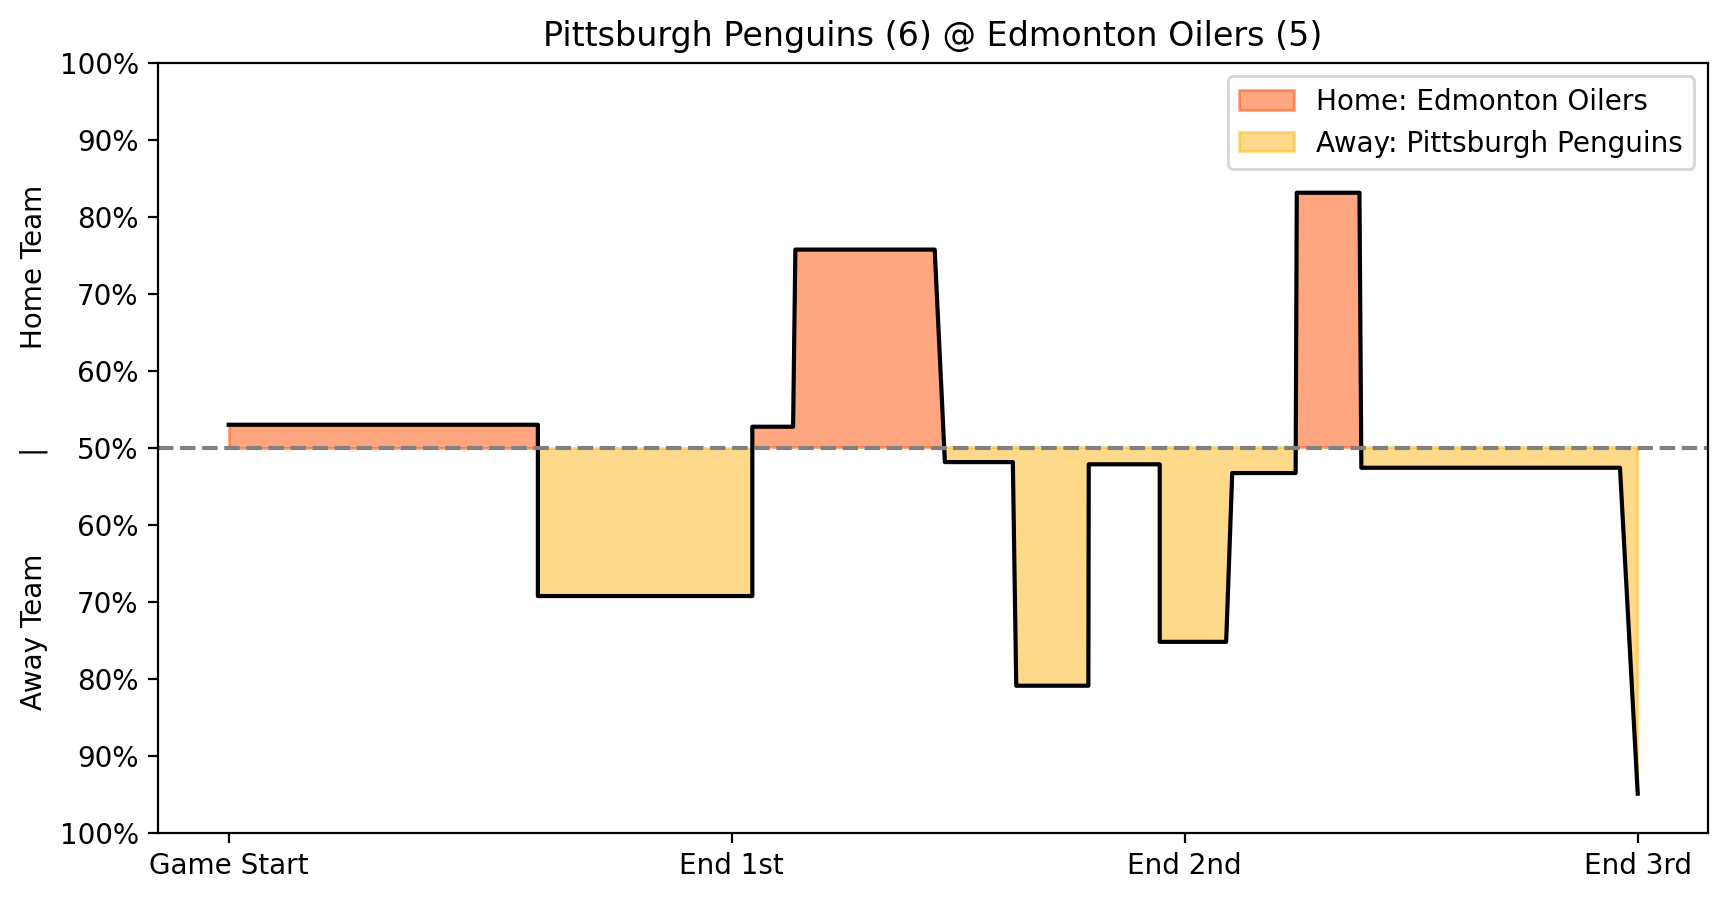
\includegraphics[width=0.9\textwidth]{images/good_bayesian_example.png}
    \caption{Win probability graph using the Bayesian Network. As seen above, the win probability stayed rather stagnant until a goal was scored, where the probability shifted.}
    \label{fig:bayesian_graph}
\end{figure}

\subsection{XGBoost}

As mentioned in the methods section, we trained an XGBoost model for each team in the NHL. One main benefit of this
approach is the ability to leverage the {\tt .predict\_proba()} method of XGBoost.
Using this method, we generated 
probabilistic predictions at various stages of a game, allowing us to 
plot the evolving probability of each team winning throughout the match
(see~\ref{fig:xgboost_res}). 
This approach provided insights into momentum shifts (when one team 
has an advantage due to them having more players on the ice due to 
a penalty by the opposing team), key moments (such as goals and 
penalties, and critical plays influencing game outcomes).

\begin{figure}[H]
    \centering
    \subfigure[]{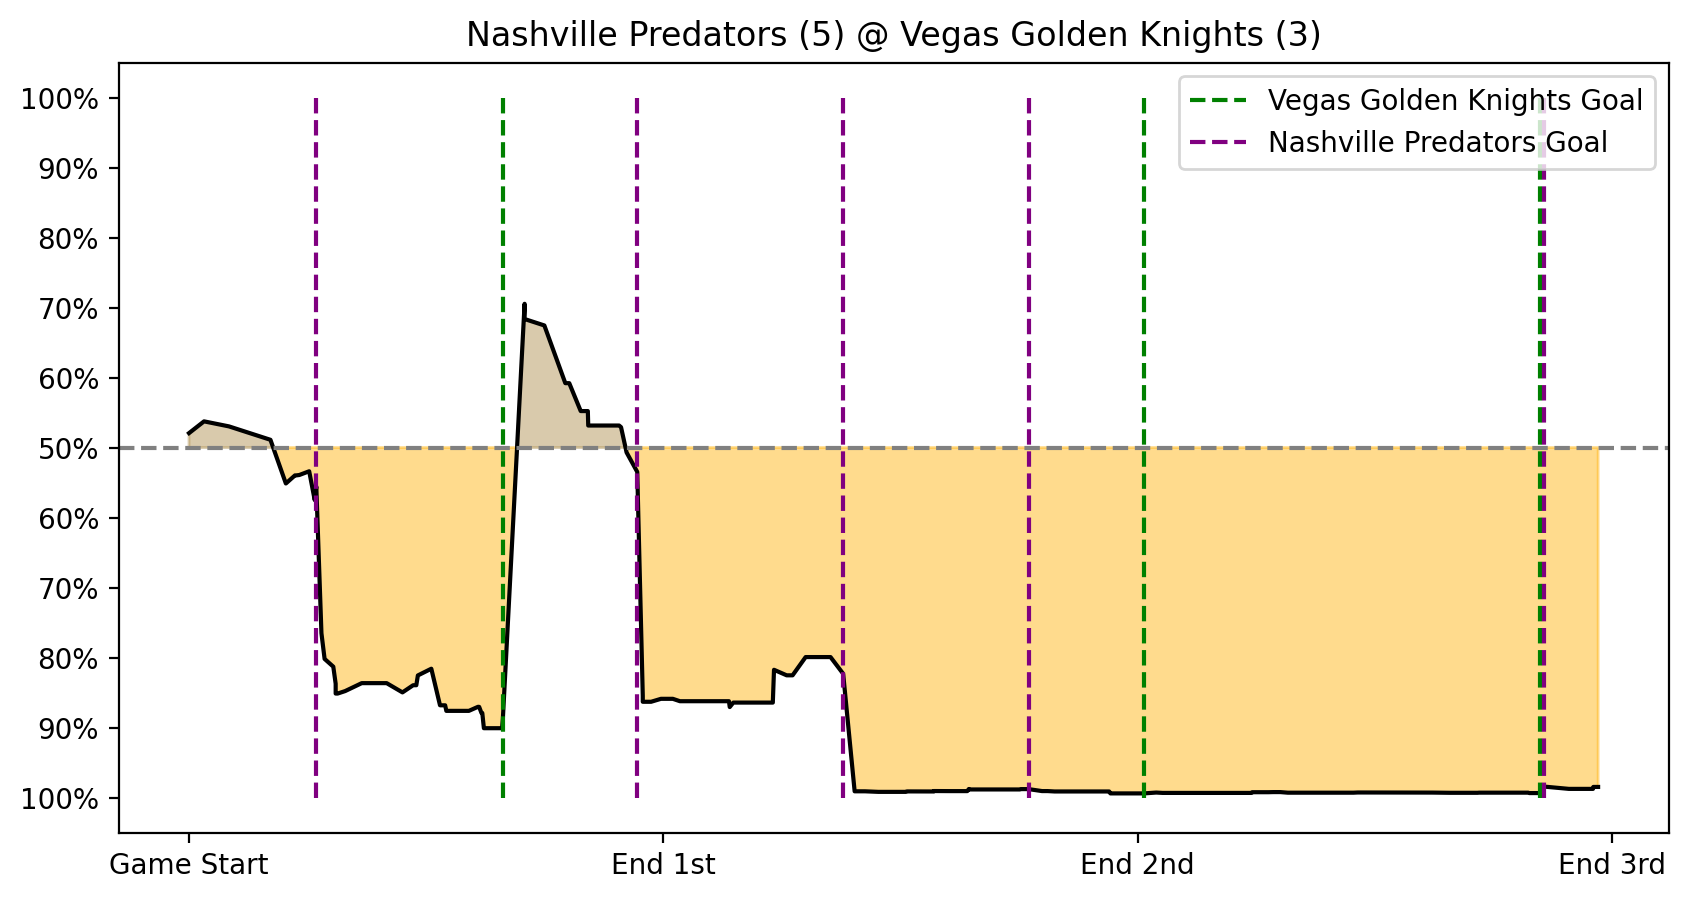
\includegraphics[width=0.6\textwidth]{images/good_xgb_example.png}} 
    \subfigure[]{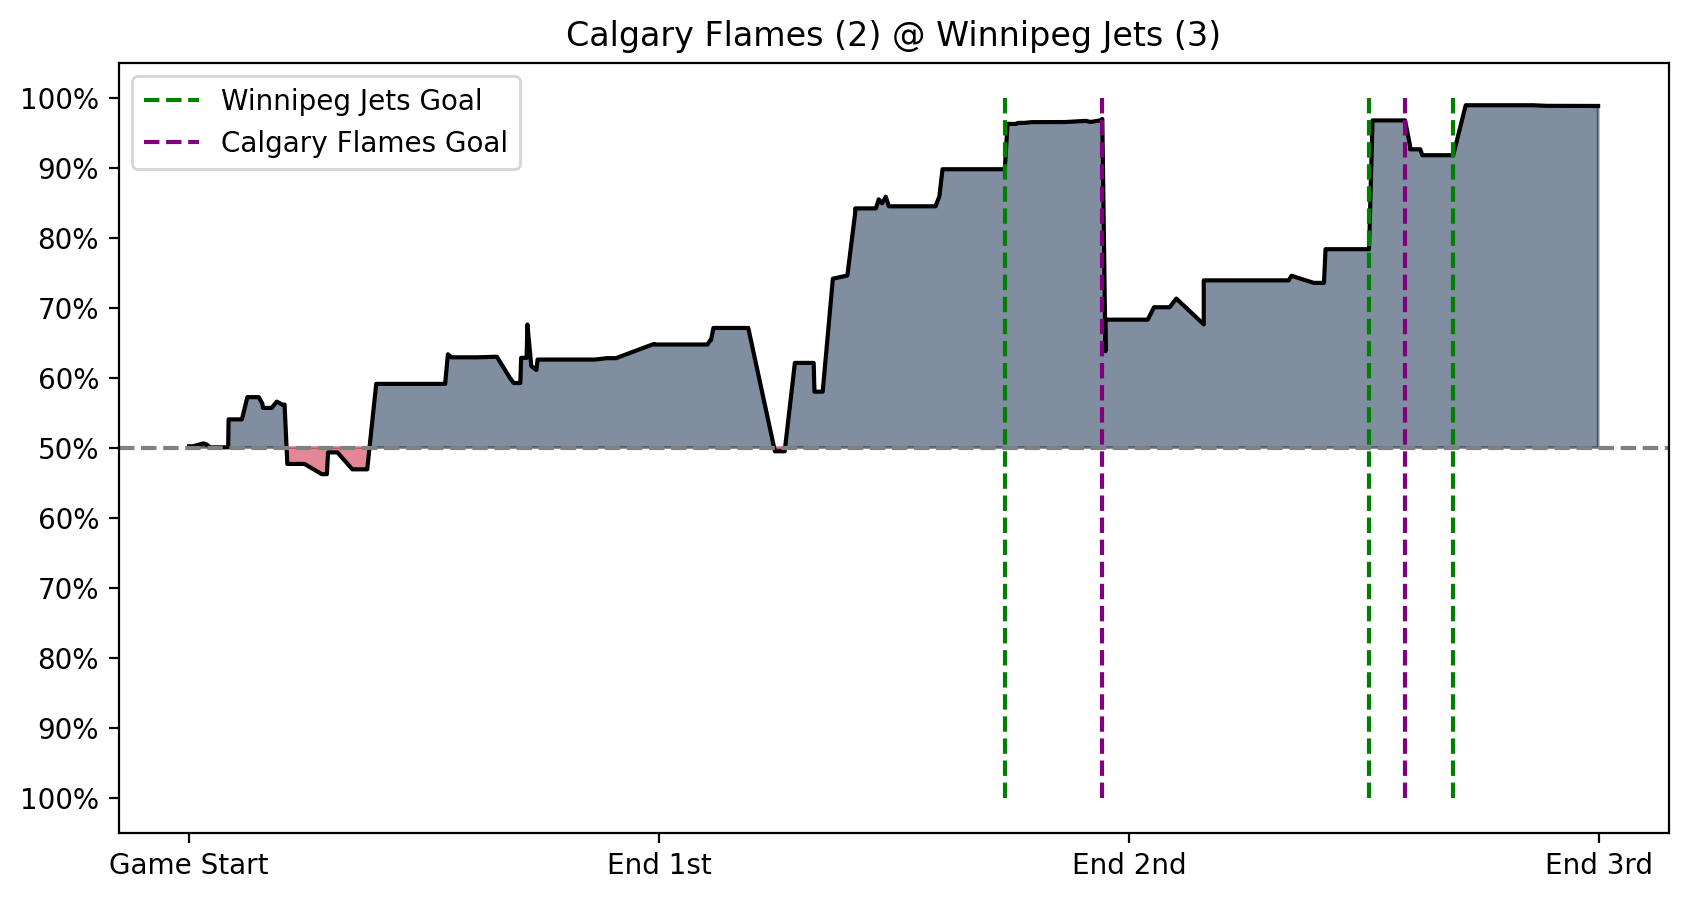
\includegraphics[width=0.6\textwidth]{images/good_xgb_example(2).png}} 
    \caption{For both of these plots, the home team is above the the 50\% line, with the
    away team below. The title has the final score of the game. \\
        \textbf{(a)} The live win probabilities for the Nashville Predators at the Vegas Golden Knights. 
    Notice the probability shifts after one team scores a goal.  \\
        \textbf{(b)} The live win probabilities for the Calgary Flames at the Winnipeg Jets.
        Notice the stark changes in probabilities after each goal. Also notice the
        shift in probabilities even when no goals are scored.}
    \label{fig:xgboost_res}
\end{figure}

\subsection{MCMC Simulator}

To evaluate our simulation's effectiveness at accurately modeling actual hockey 
games, we combined a dataset with the final event counts for 1500 actual hockey 
games and for 1500 simulated games. We then performed two experiments. First, We 
trained a KMeans, Logistic Regression, RandomForest and XGBoost model on this 
dataset with default parameters, to see 
if they could classify games as simulated or real. With a 70-30 train-test split, 
the accuracies on the test set were 47.9\%, 48.5\%, 67.5\% and 69.3\% respectively. 
Second, we fit and transformed this dataset using PCA, t-SNE and UMAP 
dimensionality reductions using various perplexity and neighbor hyperparameters to see 
if these algorithms clustered the synthetic games and actual games in 
different clusters. As shown below in ~\ref{fig:simulation_v_actual}, the simulated
games and actual games are all clustered together. From these two experiments, we conclude
that our simulator effectively models live NHL games.

\begin{figure}[H]
    \centering
    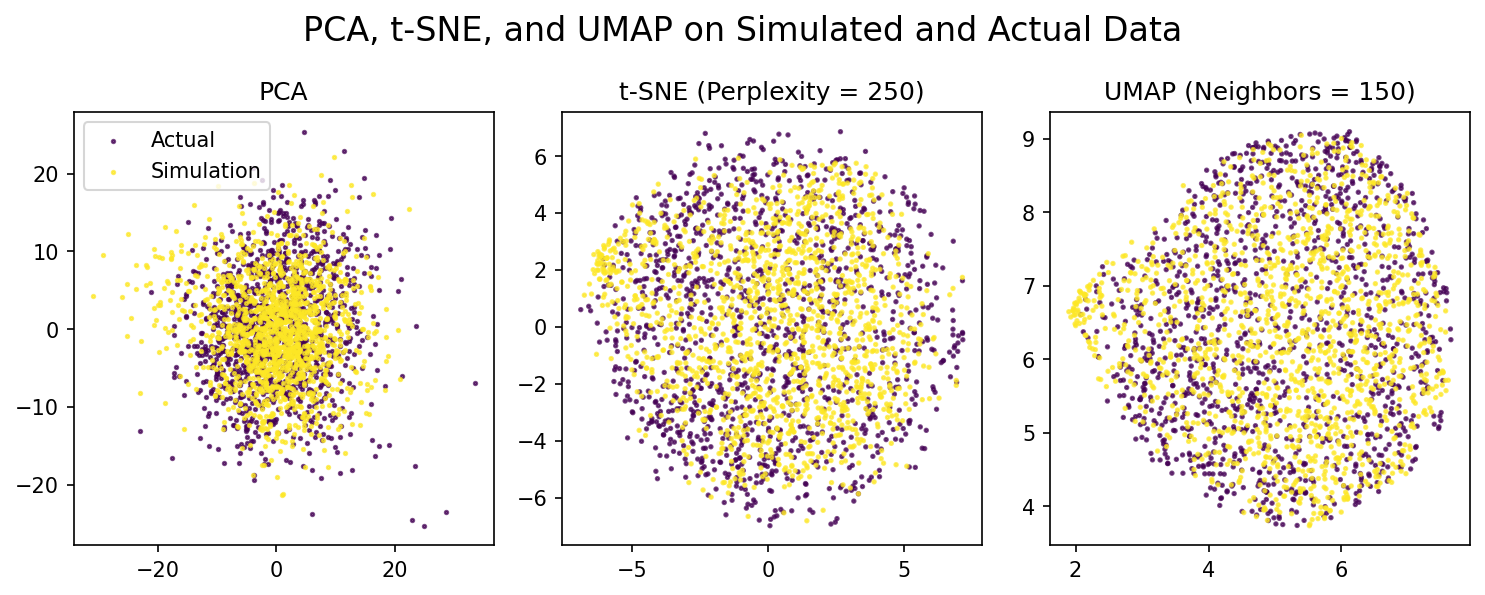
\includegraphics[width=0.9\textwidth]{images/pca_tsne_umap_sim_act.png}
    \caption{PCA, t-SNE, and UMAP performed on a dataset with final event counts for 1500 simulated and 1500 actual NHL games. The joined grouping demonstrates that our simulation accurately emulates live NHL games. Note that we performed the t-SNE and UMAP on many different values of perplexity and neighbors, but all of the plots looked the same, so we just show this one}
    \label{fig:simulation_v_actual}
\end{figure}

\subsection{Method Comparison}
Each of the methods described above had one general purpose: accurately predict the outcome of a hockey game regardless of the point in the game. To evaluate our models, we randomly selected 50 games outside of the training data, and for various time steps throughout these games we had each model calculate a win probability. We then used the probability threshold of 0.5 to determine whether or not each model predicted if the home team won or lost. We then computed each model's accuracy across all 50 games for each of the time steps.

\begin{figure}[H]
    \centering
    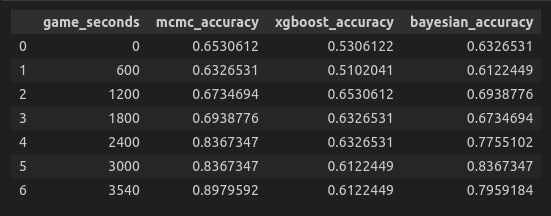
\includegraphics[width=0.9\textwidth]{images/game_accuracies.png}
    \caption{Each of our model's predictive accuracy over the course of 50 games}
    \label{fig:game_accuracies}
\end{figure}

In figure ~\ref{fig:game_accuracies} we note that each model increased in accuracy as the game progressed. We also notice that the MCMC simulation method appears to have the highest accuracy regardless of the point in the game while XGBoost appears to be the least accurate. We infer that the XGBoost models were overfit, since they appeared to perform very well on games within the training set. Also, during experimentation with the models, we noticed that the MCMC simulator and the Bayesian Network tended to produce higher probabilities for the away team winning, and the XGBoost model tended to give higher probabilities to the home team winning. The MCMC and Bayesian Network are structured to model the flow of events, so it appears that they picked up on a more predictive flow in how away teams play.

\section{Ethical Considerations}
Predicting win percentages or outcomes in hockey games, like any sport, raises several ethical considerations. Here are some key points we want to address:

\begin{itemize}[label=\textbullet]
\item \textbf{Gambling and Addiction}:
Our win percentages and predictions might be used by those who wish to gamble, which could lead to addiction and financial harm, especially if undue trust in placed in these methods. Any publication of these methods or predictions would be accompanied by promoting healthy and responsible gambling practices.
    
\item \textbf{Fairness and Integrity of the Game}:
Sometimes, coaches and players becoming aware of their chance of winning can affect how the game is played, potentially harming the integrity of the sport. We must be careful to not provide an unfair advantage to any team or player.
Inaccurate predictions could lead a team to believe that the game is out of reach when it isn't, and we want to avoid that.
            
\end{itemize}

Overall, our predictions, like any, should not be considered declarative for gambling or performance purposes, but are rather an interesting exposition into the complexity of sporting events.


\section{Conclusion}

In this project, we used three different methods to predict the outcomes of NHL games. We used a Bayesian Network to model the conditional dependencies of key features, XGBoost to model the play-by-play dynamics of each team, and an MCMC simulator to simulate the flow of events in a hockey game. We found that the MCMC simulator was the most accurate, with the Bayesian Network coming in second, and XGBoost coming in last. 
The win percentages predicted are more for entertainment and educational purposes, and should not be used for gambling or performance purposes, as they do not have a incredibly high degree of accuracy. There are many variables in a hockey game that affect win probability, and given more time and more data we would love to model other factors such as momentum, historical success, coaching, etc. Our project was limited by the data
we had access to and computational resources, but nonetheless we were able to produce a model that can predict the outcome of NHL games with a reasonable degree of accuracy.

% new page
\newpage

% Bibliography
\bibliographystyle{plain}
\bibliography{references} % Replace 'references' with the name of your .bib file

\end{document}

